\FrontMatter{Introduction}
This introduction shows the workbook voice and layout. The class provides convenient color-switching
macros such as {\blue blue text}, {\maroon maroon text}, and {\lake lake-colored text}. It also
provides an emphasis macro: \alert{important ideas can be highlighted consistently}. Throughout the
template, cross-references use \verb|\cref|, for example \cref{thm:derivative-power,def:inner-product}.

\begin{center}
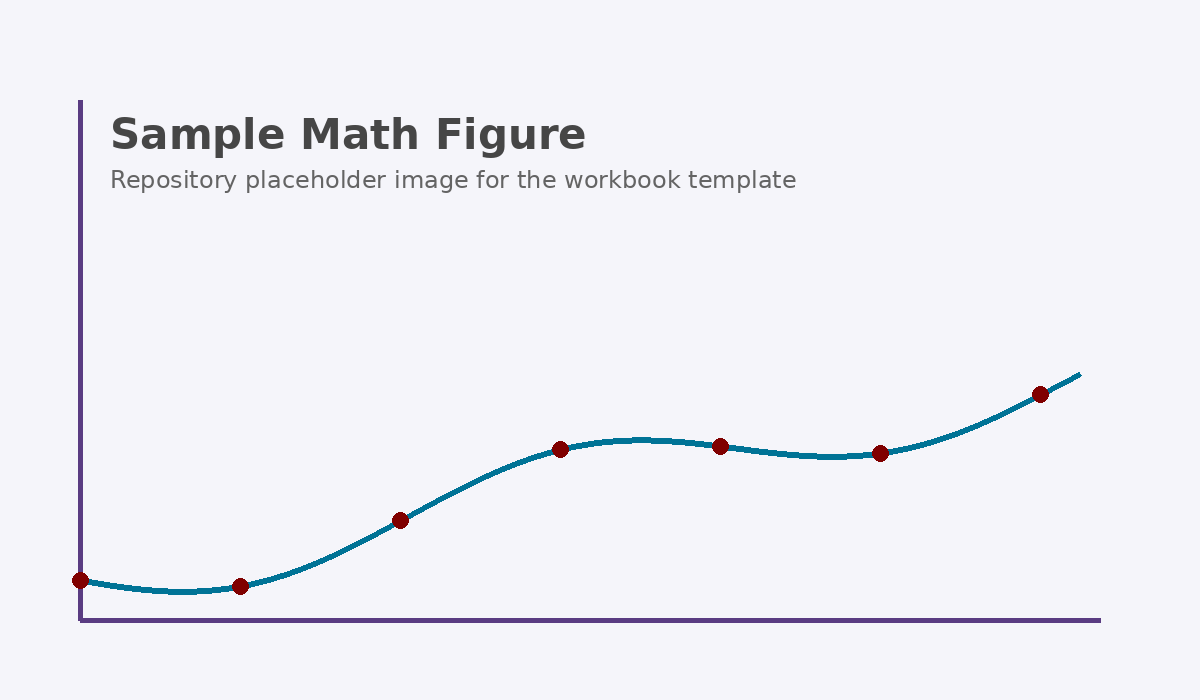
\includegraphics[width=0.55\linewidth]{images/sampleimage.png}
\end{center}

\chapterline{maroon}{88}

\section{Repository structure}
The top-level file \texttt{main.tex} compiles the workbook. The folder \texttt{chapters/} stores modular
chapter files, \texttt{appendices/} stores appendices, and \texttt{assignments/} stores standalone
worksheet-mode assignments. The command \verb|\blankfill| is useful for fill-in-the-blank prompts:
Course website \blankfill

\begin{note}[Template note:]
This note box shows one recommended use of the class: keep exposition in workbook mode and use the
worksheet option for short assignments or handouts.
\end{note}

\begin{warning}[Compilation reminder:]
Because the class uses \texttt{biblatex} with the \texttt{biber} backend, the workbook should be compiled
with a LaTeX $\to$ Biber $\to$ LaTeX $\to$ LaTeX workflow.
\end{warning}

\begin{digression}
A compact workbook often benefits from short historical or conceptual side paths. This environment is a
natural place to discuss why a result matters before returning to the main thread.
\end{digression}

\begin{lectureplan}[Opening module]
\planhead{Learning Objectives}
Students should recognize the repository layout, identify the main entry points, and understand how the
class structures theorem-like environments.

\planhead{Timing (10 minutes)}
Spend a few minutes walking through the folder structure and the sample chapter files.
\end{lectureplan}

\begin{staffnote}[Instructor note:]
The lecture-plan and staff-note environments are most useful in instructor-facing copies of the workbook.
Set \texttt{\string\showplanfalse} in a student-facing version if you want to suppress them.
\end{staffnote}
